\documentclass{article}
\usepackage{graphicx}
\usepackage{amsmath}
\usepackage{gensymb}
\usepackage{indentfirst}
\usepackage[UKenglish]{isodate}

\author{Athena Boose\\Reed Fowler\\Justin Joy\\Dylan Orozco\bigskip\\Physics 188}
\date{\today}
\title{Lab 7 Report - Group 7}

\begin{document}
\cleanlookdateon
\maketitle

\section{Goal}

\noindent The goal of this lab was to do the following:

\begin{itemize}
    \item Measure the orbital velocity of matter in the Milky Way
    \item Measure the mass of the Milky Way that resides within certain radii
    \item Determine whether the mass of the Milky Way is concentrated predominately within its center or whether this mass is spread out throughout the galaxy's disk
    \item Determine whether the Milky Way is predominately composed of visible or dark matter
\end{itemize}

\section{Skills Learned}

\noindent We learned the following skills during this exercise:

\begin{itemize}
    \item How to use Skynet to take radio observations using Green Bank Observatory's radio telescope
    \item How to use the data from these radio observations to determine both the orbital velocity of regions of the Milky Way as well as the distance of these regions from the center of the Milky Way
    \item How to plot the velocity of regions of the Milky Way against their distance from the center of the Milky Way, as well as how to use this plot to determine where the mass of the Milky Way is concentrated
    \item How to determine the mass of objects in the Milky Way that orbit below a certain radius
    \item How to use the orbital velocity of and distance from the center of the Milky Way of the Large and Small Magellanic Clouds to determine whether Dark or Visible matter is more prevalent in the Milky Way
\end{itemize}

\section{Data Collected}

\noindent The following data was collected:

\begin{itemize}
    \item Radio spectra at roughly 21.1 cm
    \begin{itemize}
        \item All spectra were collected at 0\degree \space galactic latitude and at 
        0\degree, 
        8\degree, 
        16\degree, 
        24\degree, 
        32\degree, 
        40\degree, 
        48\degree, 
        56\degree, 
        64\degree, 
        72\degree, 
        80\degree, and 
        88\degree galactic longitude.
    \end{itemize}
\end{itemize}

\noindent The following data was provided and used in our analysis:

\begin{itemize}
    \item Hydrogen emission line \\ $\lambda_{em}=21.1061$ cm
    \item Speed of light \\ $c=3.00\cdot10^5$ km/s
    \item Orbital velocity of the Sun around the center of the Milky Way \\ $V_{sun}=220$ km/s
    \item Distance of the Sun from the center of the Milky Way \\ $R_{sun}=8.1$ kpc
    \item Orbital velocity of the Large and Small Magellanic clouds around the center of the Milky Way
    \item Distance of the Large and Small Magellanic clouds from the center of the Milky Way
    \item Gravitational constant $G=4302\text{ }\frac{(\text{km/s})^2 \cdot kpc}{GM_{sun}}$
\end{itemize}

\section{Analysis of Data}

\subsection{Calculation of Orbital Velocity of Matter in the Milky Way}

To calculate the orbital velocity of matter in the Milky Way, we first had to calculate the velocity of this matter relative to the Sun.
This can be done using the following equation:

\[
\Delta V = c \cdot \frac{\lambda_{obs} - \lambda_{em}}{\lambda_{em}}
\]

where $c = 3.00 \cdot 10^5$ is the speed of light, $\lambda_{em} = 21.1061$ cm is an emission line of Hydrogen, $\lambda_{obs}$ is the most-redshifted Hydrogen emission line in the observed spectrum (see Figure 1), and $\Delta V$ is the relative velocity of the observed matter.

Next, to find the orbital velocity of matter in the Milky Way given its velocity relative to the sun, the following equation can be used:

\[
V = \Delta V + V_{sun} \cdot \sin(\ell)
\]

where $V$ is the orbital velocity of the matter, $\Delta V$ is the velocity of the matter relative to the Sun, $V_{sun} = 220$ km/s is the orbital velocity of the Sun around the center of the Milky Way, and $\ell \in \{0, 8, 16, 24, 32, 40, 48, 56, 64, 72, 80, 88\}$\degree \space is the galactic longitude at which the observation was taken.

\subsection{Calculation of Orbital Radius of Matter in the Milky Way}

To calculate the orbital radius of matter in the Milky Way, the following equation can be used:

\[
R = R_{sun} \cdot \sin (\ell)
\]

Once both the orbital velocity and distance from the center of the Milky Way are known, a plot can be created (Figure 2) and examined to determine where the mass of the Milky Way is concentrated.

\subsection{Determining Whether the Milky Way is Predominately Composed of Dark Matter}

To determine whether the matter in the Milky Way is mostly composed of dark matter, it was necessary to find the amount of matter in the Milky Way enclosed within a certain radius.
To do this, the following equation can be used:

\[
M_{<R} = \frac{V^2R}{G}
\]

where $M_{<R}$ is the mass in the Milky Way within a certain radius $R$, $V$ is the orbital velocity of gas at that distance from the Milky Way, and $G=4302\text{ }\frac{(\text{km/s})^2 \cdot kpc}{GM_{\odot}}$

Once the mass enclosed within certain radii has been calculated, the radii and their associated masses can be plotted on a graph (Figure 3).

\pagebreak

\section{Figures}
\begin{center}
    \begin{figure}[h!]
        \caption{
            This is a graph of the radio emissions from 21.085-21.125 cm recorded at a Galactic Latitude of 0\degree \space and a Galactic Longitude of 88\degree \space.
            Given this graph, it is possible to find the most-redshifted emission line by finding the peak with the highest wavelength.
            These peaks can then be used to find the orbital velocity of the part of the Milky Way in the path of this observation that is closest to the center of the Milky Way.
            This orbital velocity can be combined with the orbital radius of the most-redshifted part of the Milky Way to form Figure 2.
            \smallskip
        }
        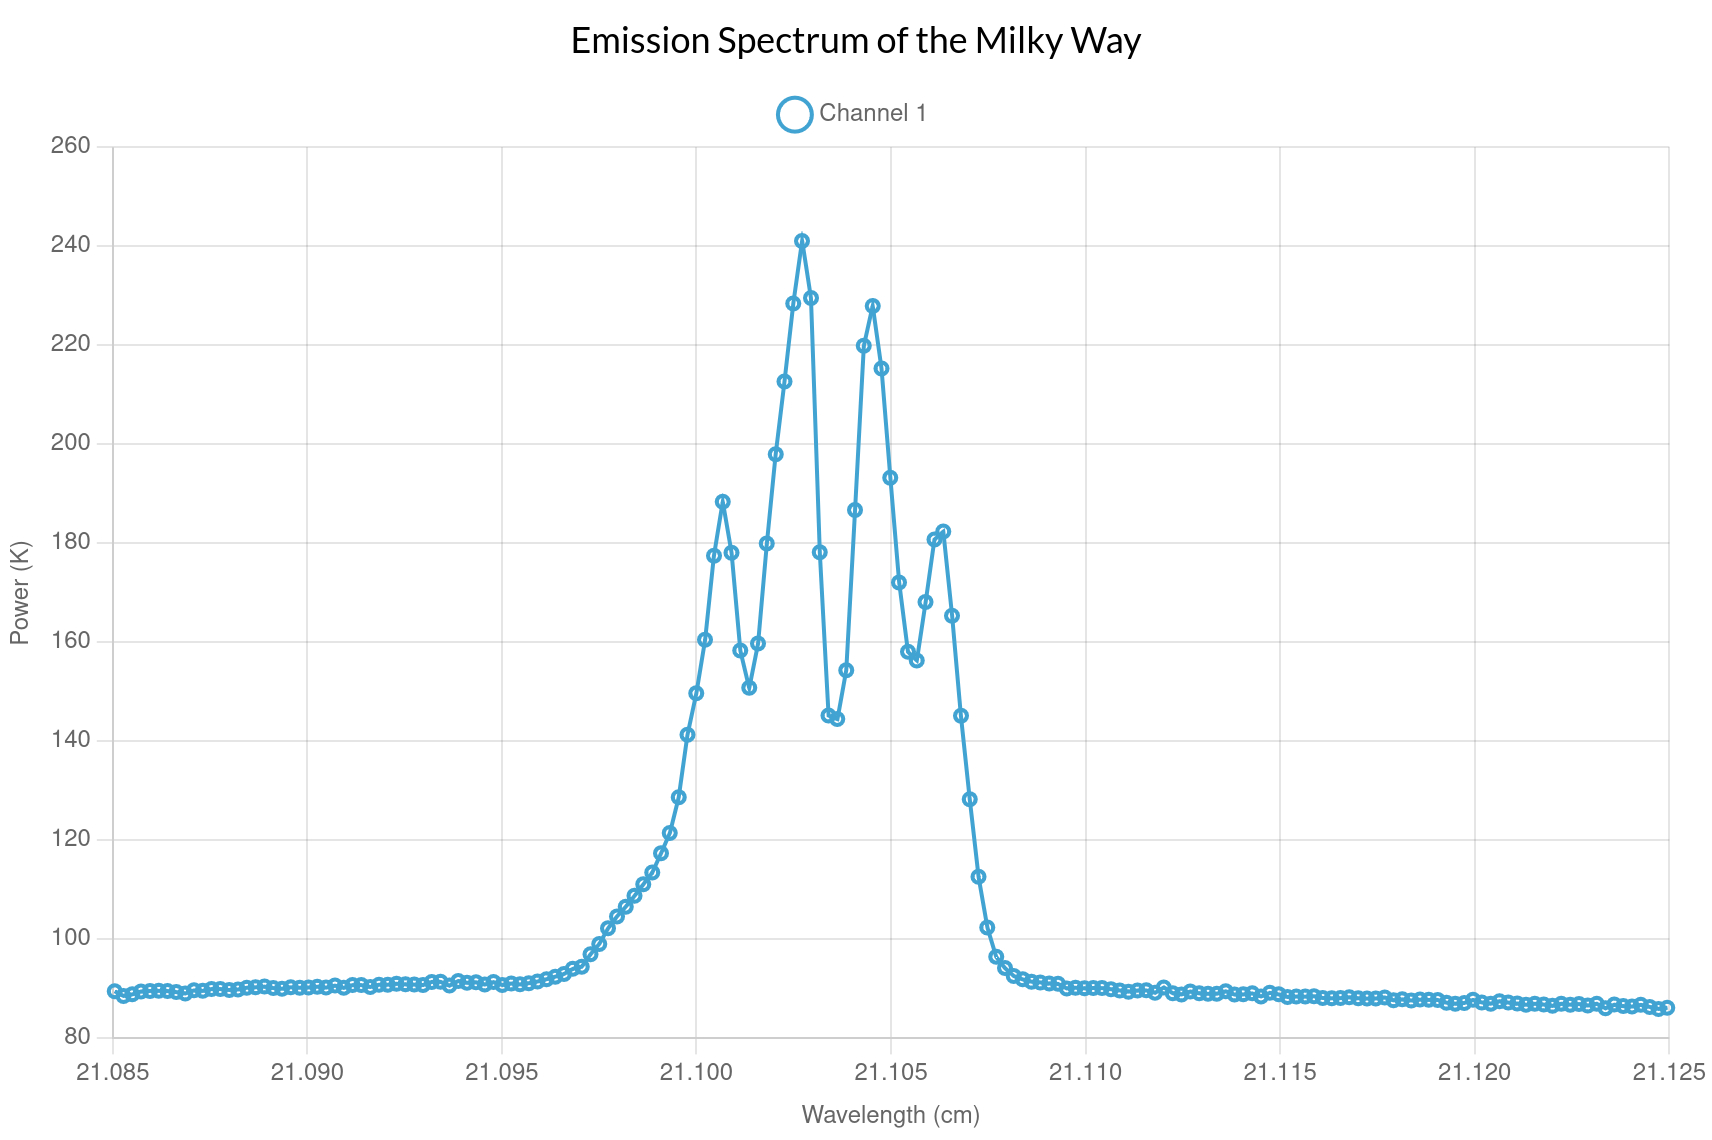
\includegraphics[scale=0.2]{emission-graph-lab9.jpg}
        \centering
    \end{figure}
    \begin{figure}[h!]
        \caption{
            This graph plots the orbital velocity of various portions of the Milky Way against their distance from the center of the Milky Way.
            Using this graph, we can conclude that the mass of the Milky Way is not all concentrated at the center of the galaxy; instead, it is spread throughout the galaxy.
            This is because the graph remains mostly constant as the orbital velocity increases, instead of decreasing as orbital velocity increases.
            \smallskip
        }
        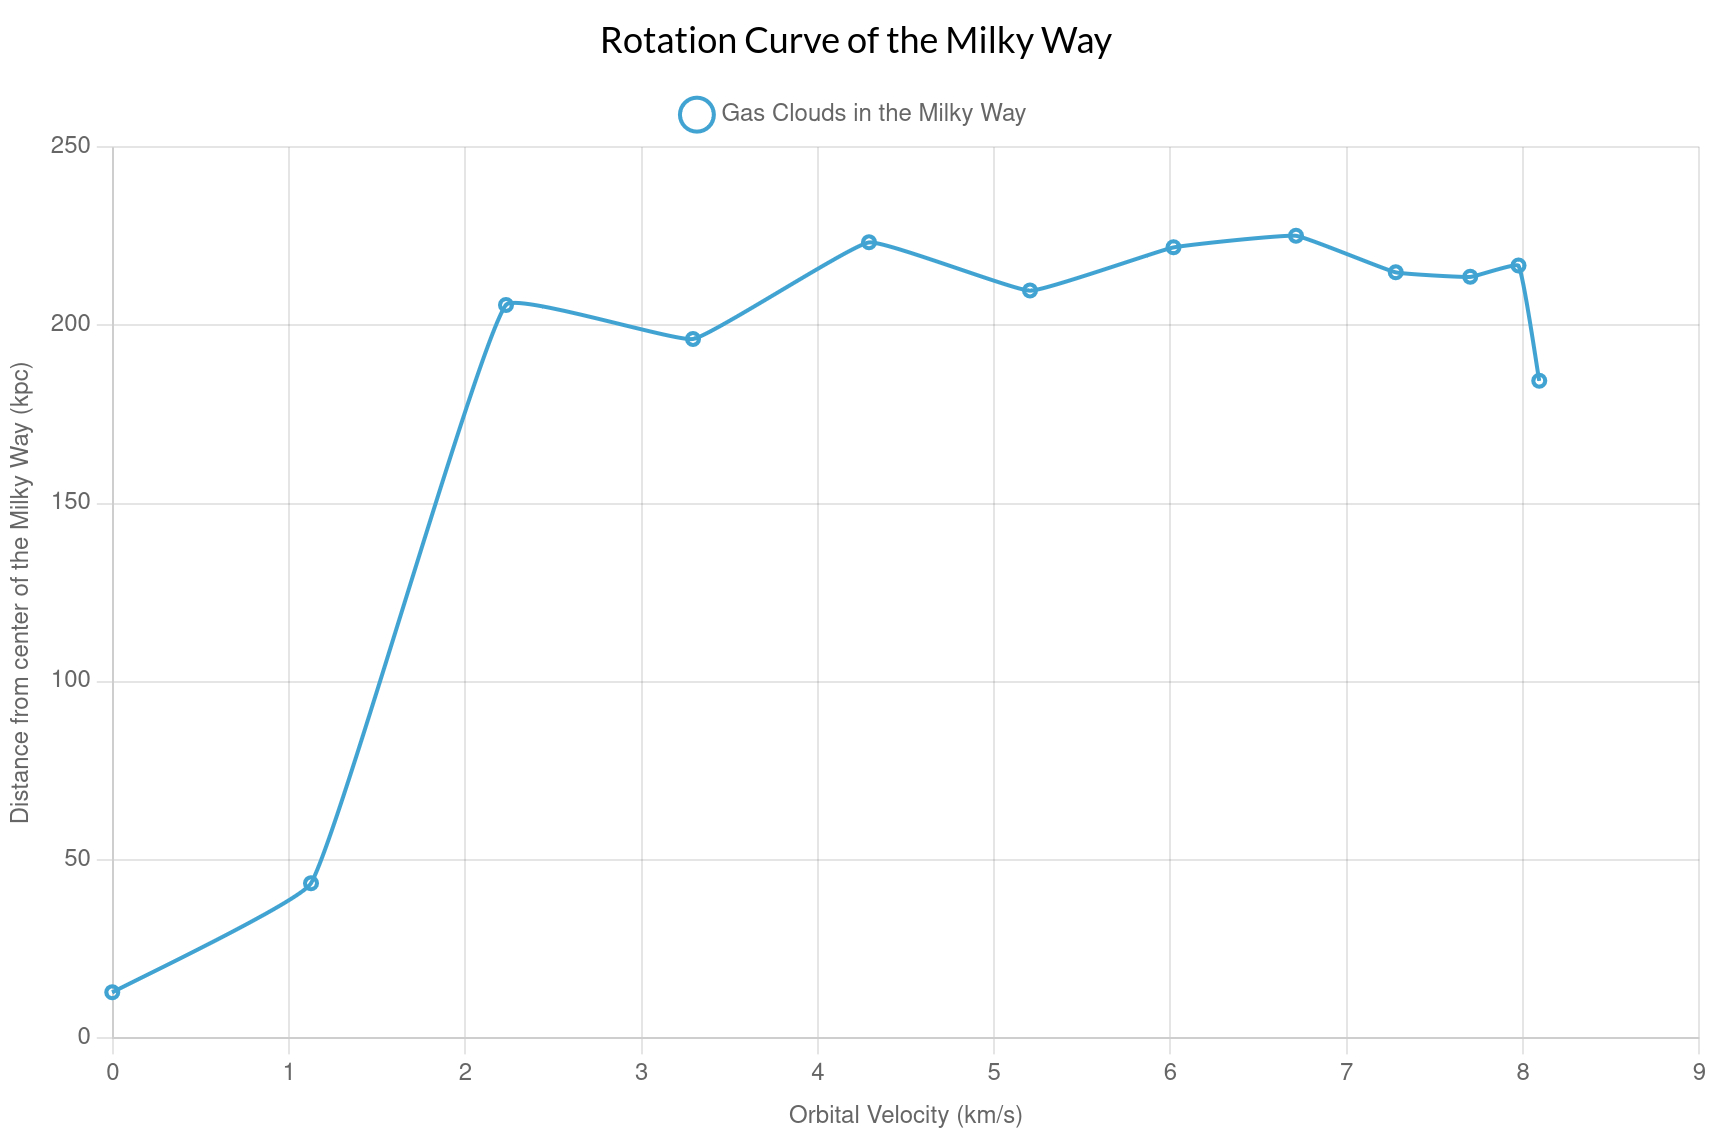
\includegraphics[scale=0.2]{rotation-curve-lab9.jpg}
        \centering
    \end{figure}
    \pagebreak
    \begin{figure}[h!]
        \caption{
            This plot relates the distance from the center of the Milky Way with the amount of mass inside that radius.
            Since the visible radius of the Milky Way is roughly 17 kpc, and the graph continues to increase beyond that point, we can conclude that there is a non-insignificant amount of Dark Matter in the Milky Way.
            \smallskip
        }
        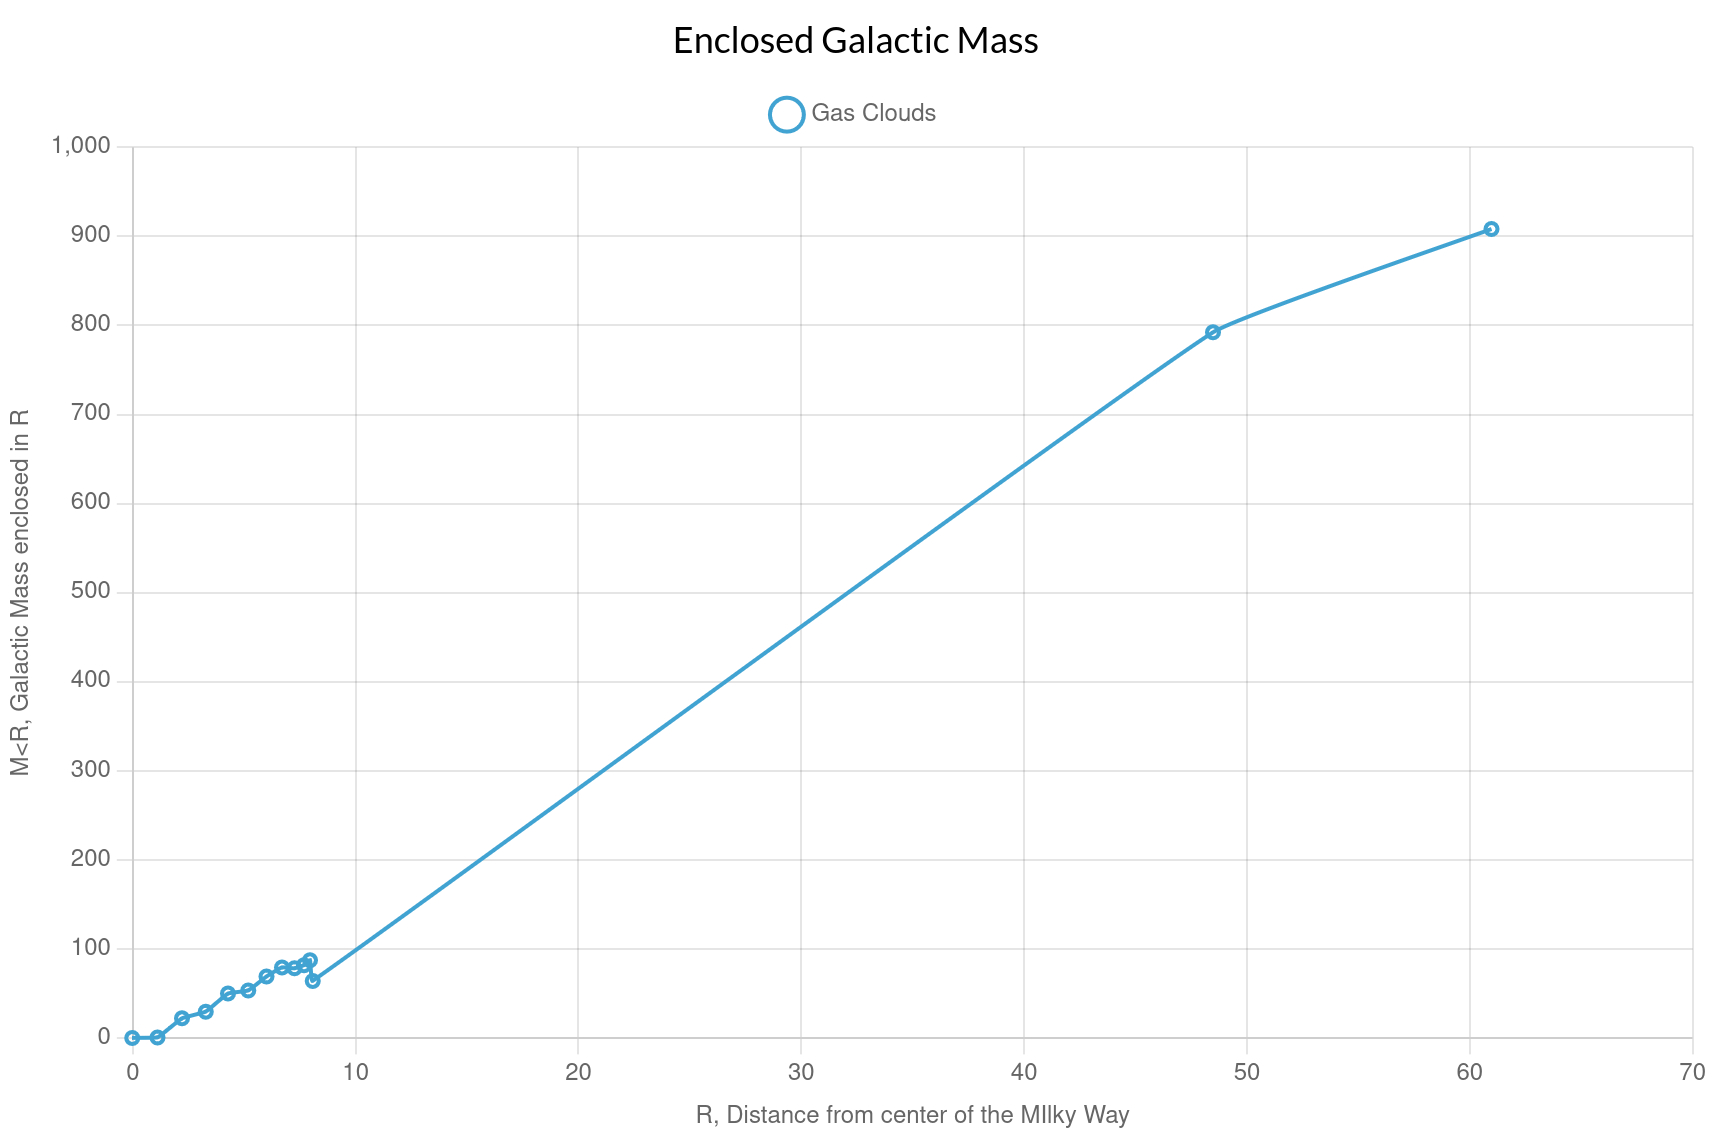
\includegraphics[scale=0.2]{distance-enclosed-mass.jpg}
        \centering
    \end{figure}
\end{center}

\pagebreak

\section{Conclusion}

Since Figure 2 does not fall off as the orbital velocity increases, the mass of the Milky Way is not concentrated in the center.

The Milky Way's visible radius is 17 kpc.
Since the mass enclosed within 17 kpc of the Milky Way's center is roughly $2.24 \cdot 10^{11}$ solar masses, and the mass enclosed within 61 kpc of the Milky Way's center is $9.0761 \cdot 10^{11}$ solar masses, we can conclude that the Milky Way is predominately composed of Dark Matter.

\section{Limitations}

\subsection{Errors}
The following factors may have impacted our ability to get accurate and/or
precise results in this lab.

\begin{itemize}
    \item Estimating the peak values of graphs 
    \item Estimating the mass of the Milky Way inside 17 kpc rather than calculating this value
    \item Velocity of Earth relative to the Sun.
\end{itemize}

\subsection{Impact of Errors}

It is likely that the impact of these errors was relatively minor, but we were not provided with the actual figures for these measurements, so we have no way to verify this other than noting that our graphs seem to be roughly correct.

\end{document}